\section{Auswertung}
\label{sec:Auswertung}

Die Graphen wurden sowohl mit Matplotlib \cite{matplotlib} als auch NumPy \cite{numpy} erstellt. 
Die Fehlerrechnung wurde mithilfe von Uncertainties \cite{uncertainties} durchgeführt.
Die Konstanten $\mu_0$, $g$ und $\pi$ sind von SciPy \cite{scipy}.
Die Werte für die Windungszahl $N$, den Abstand $d$, und den Radius $R$ der Helmholzspule sind:
\begin{align*}
N &= 195\\
d &= \SI{13,8}{\centi\metre}\\
R &= \SI{10,9}{\centi\metre}
\end{align*}

\subsection{Bestimmung des magnetischen Momentes unter Ausnutzung der Gravitation}

Mithilfe der Messwerte für $I$ aus Tabelle \ref{tab:Gravitation} werden mit Formel \eqref{eq:B} die jeweiligen magnetischen Flussdichten $B$ für die verschiedenen Abstände $r$ der Masse $m=\SI{1,4}{\gram}$ vom Ursprung der Kugel bestimmt. Es wird $r$ gegen $B$ aufgetragen (vgl. Graph \ref{fig:Gravitation}) und mittels Formel \eqref{eq:??} das magnetische Moment $\mu_.{Dipol}$ der Kugel bestimmt zu:
\begin{equation*}
\mu_.{Dipol} = \SI{0,437(6)}{\ampere\per\metre\squared}
\end{equation*}  
\begin{table}
  	\centering
  	\caption{Die Messwerte von $r$ und $I$ der ersten Messreihe, sowie die berechneten Werte für $B$.}
  	\label{tab:taba}
	\sisetup{table-format=1.2}
	\begin{tabular}{S[table-format=1.1]S[table-format=1.2]S[table-format=1.2]}
		\toprule
		{$r/\si{\centi\metre}$} & {$I/\si[per-mode=reciprocal]{\ampere}$} & {$B/\si[per-mode=reciprocal]{\milli\tesla}$} \\
		\midrule
		4.6 & 1.25 & 1.70 \\
		5.1 & 1.39 & 1.88 \\
		5.6 & 1.49 & 2.02 \\
		6.1 & 1.61 & 2.18 \\
		6.6 & 1.71 & 2.32 \\
		7.1 & 1.81 & 2.45 \\
		7.6 & 1.95 & 2.64 \\
		8.1 & 2.09 & 2.83 \\
		8.6 & 2.19 & 2.97 \\
		9.1 & 2.29 & 3.11 \\
		\bottomrule
	\end{tabular}
\label{tab:Gravitation}
\end{table}
\begin{figure}
	\centering
	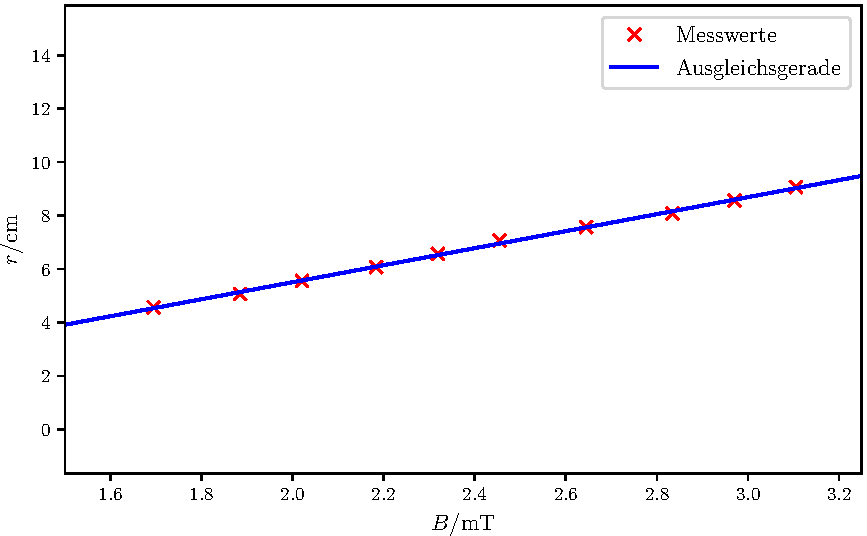
\includegraphics[scale = 1,keepaspectratio]
	{content/images/Gravitation.pdf}
	\caption{Verlauf von $r$ in Abhängigkeit von $B$}
	\label{fig:Gravitation}
\end{figure}
\subsection{Bestimmung des magnetischen Momentes über die Schwingungsdauer}

Mithilfe der Messwerte für $I$ aus Tabelle \ref{tab:Schwingungsdauer} werden mit Formel \eqref{eq:B} die jeweiligen magnetischen Flussdichten $B$ bestimmt. Das Trägheitsmoment $I_.K$ der Kugel mit Radius $r_.K = \SI{2,66}{\centi\metre}$ und Masse $m_.K = \SI{142}{\gram}$ beträgt nach Formel \eqref{eq:??}:
\begin{equation*}
I_.K = \SI{4,03e-5}{\kilogram\metre\squared}
\end{equation*}
Es wird $T^2$ gegen $1/B$ aufgetragen (vgl. Graph \ref{fig:Schwingungsdauer}) und mittels Formel \eqref{eq:??} das magnetische Moment $\mu_.{Dipol}$ der Kugel bestimmt zu:
\begin{equation*}
\mu_.{Dipol} = \SI{0,438(10)}{\ampere\per\metre\squared}
\end{equation*}  
\begin{table}
  	\centering
  	\caption{Die Messwerte von $I$ und $T$ der zweiten Messreihe, sowie die berechneten Werte für $B$.}
  	\label{tab:tabb}
	\sisetup{table-format=1.2}
	\begin{tabular}{S[table-format=5.0]S[table-format=2.2]S[table-format=2.2]S[table-format=1.2]S[table-format=1.2]}
		\toprule
		{$f/\si{\hertz}$} & {$U/\si{\volt}$} & {$\frac{U}{U_0}$} & {$a/10^{-4}\si{\second}$} & {$\phi/\si{\radian}$} \\
		\midrule
		   10 & 96.00 & 1.00 & 6.00 & 0.04 \\
		   30 & 94.00 & 0.98 & 6.00 & 0.11 \\
		   70 & 90.00 & 0.94 & 6.00 & 0.26 \\
		  100 & 86.00 & 0.90 & 7.60 & 0.48 \\
		  200 & 66.40 & 0.69 & 6.20 & 0.78 \\
		  300 & 52.00 & 0.54 & 5.20 & 0.98 \\
		  500 & 34.40 & 0.36 & 3.00 & 0.94 \\
		  700 & 25.20 & 0.26 & 3.00 & 1.32 \\
		 1000 & 17.40 & 0.18 & 2.30 & 1.45 \\
		 2000 & 8.00 & 0.08 & 1.20 & 1.51 \\
		 3000 & 4.88 & 0.05 & 0.78 & 1.47 \\
		 4000 & 3.28 & 0.03 & 0.59 & 1.48 \\
		 5000 & 2.24 & 0.02 & 0.47 & 1.48 \\
		 6000 & 1.64 & 0.02 & 0.40 & 1.51 \\
		 7000 & 1.20 & 0.01 & 0.34 & 1.50 \\
		 8000 & 0.84 & 0.01 & 0.30 & 1.51 \\
		10000 & 0.34 & 0.00 & 0.25 & 1.57 \\
		\bottomrule
	\end{tabular}
\label{tab:Schwingungsdauer}
\end{table}
\begin{figure}
	\centering
	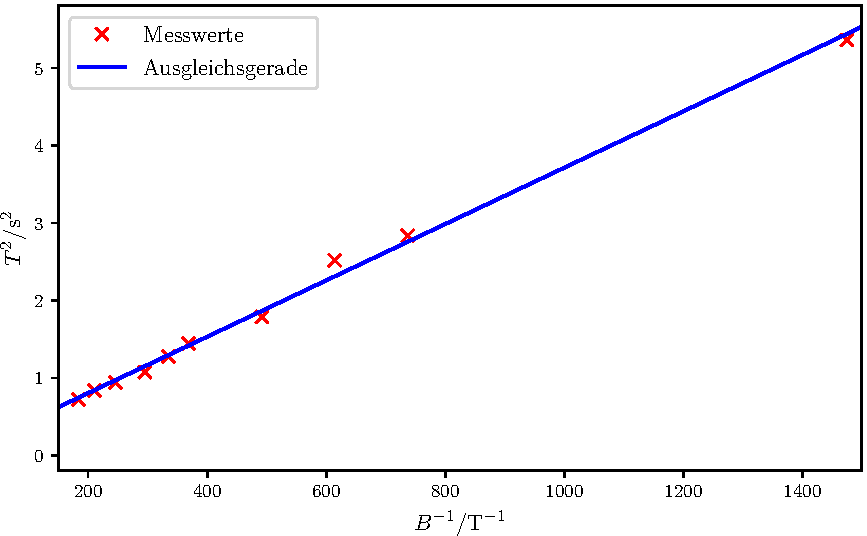
\includegraphics[scale = 1,keepaspectratio]
	{content/images/Schwingungsdauer.pdf}
	\caption{Verlauf von $T^2$ in Abhängigkeit von $1/B$}
	\label{fig:Schwingungsdauer}
\end{figure}

\subsection{Bestimmung des magnetischen Momentes über die Präzession}

Mithilfe der Messwerte für $I$ aus Tabelle \ref{tab:Präzession} werden mit Formel \eqref{eq:B} die jeweiligen magnetischen Flussdichten $B$ bestimmt. Der Drehimpuls $L_.K$ der Kugel kann mit Formel \eqref{eq:??} bestimmt werden zu:
\begin{equation*}
L_.K = \SI{1,27}{\gram\metre\squared\per\second}
\end{equation*}
Es wird die reziproke Zeit $T^{-1}$ gegen $B$ aufgetragen (vgl. Graph \ref{fig:Präzession}) und mittels Formel \eqref{eq:??} das magnetische Moment $\mu_.{Dipol}$ der Kugel bestimmt zu:
\begin{equation*}
\mu_.{Dipol} = \SI{0,363(11)}{\ampere\per\metre\squared}
\end{equation*}  
\begin{table}
  	\centering
  	\caption{Die Messwerte von $I$ und $T$ der dritten Messreihe, sowie die berechneten Werte für $B$.}
  	\label{tab:tabc}
	\sisetup{table-format=1.2}
	\begin{tabular}{S[table-format=1.1]S[table-format=1.1]S[table-format=2.2] @{${}\pm{}$} S[table-format=1.2]}
		\toprule
		{$I/\si{\ampere}$} & {$B/\si[per-mode=reciprocal]{\milli\tesla}$} & \multicolumn{2}{c}{$T/\si[per-mode=reciprocal]{\second}$} \\
		\midrule
		0.5 & 0.7 & 23.51 & 0.39 \\
		1.0 & 1.4 & 14.44 & 0.34 \\
		1.2 & 1.6 & 11.78 & 0.29 \\
		1.5 & 2.0 & 10.15 & 0.09 \\
		2.0 & 2.7 & 8.12 & 0.24 \\
		2.2 & 3.0 & 7.36 & 0.16 \\
		2.5 & 3.4 & 5.87 & 0.08 \\
		3.0 & 4.1 & 4.99 & 0.07 \\
		3.5 & 4.7 & 4.39 & 0.05 \\
		4.0 & 5.4 & 3.98 & 0.04 \\
		\bottomrule
	\end{tabular}
\label{tab:Präzession}
\end{table}
\begin{figure}
	\centering
	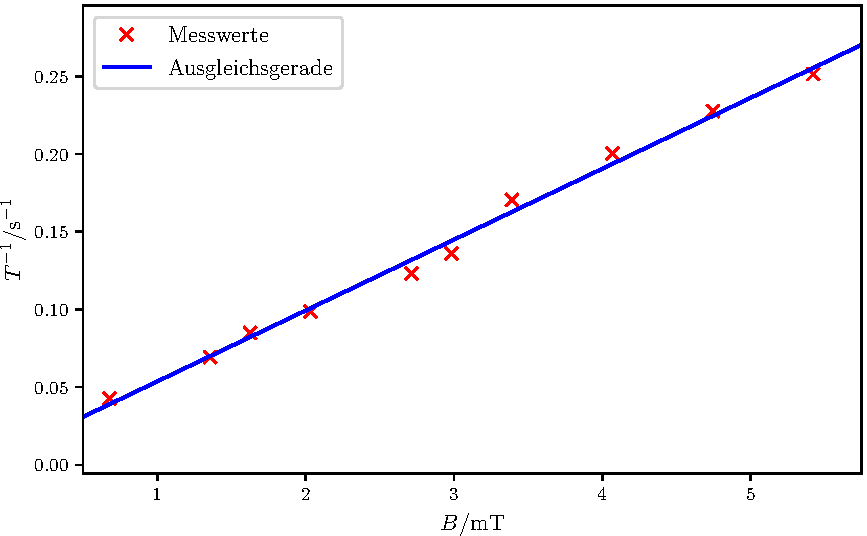
\includegraphics[scale = 1,keepaspectratio]
	{content/images/Praezession.pdf}
	\caption{Verlauf der reziproken Zeit $T^{-1}$ in Abhängigkeit von $B$}
	\label{fig:Präzession}
\end{figure}